% !TEX root = ../Report.tex

overview

\subsection{LUNA16 dataset}

The used dataset is from the LUNA16 challenge and each scan contains a number of slices. The algorithm creates a label map for each slice marking every pixel that is part of the lung. An example of one scan and the corresponding labeling is shown in figure \ref{scan_picture}.

\begin{figure}[h!]
	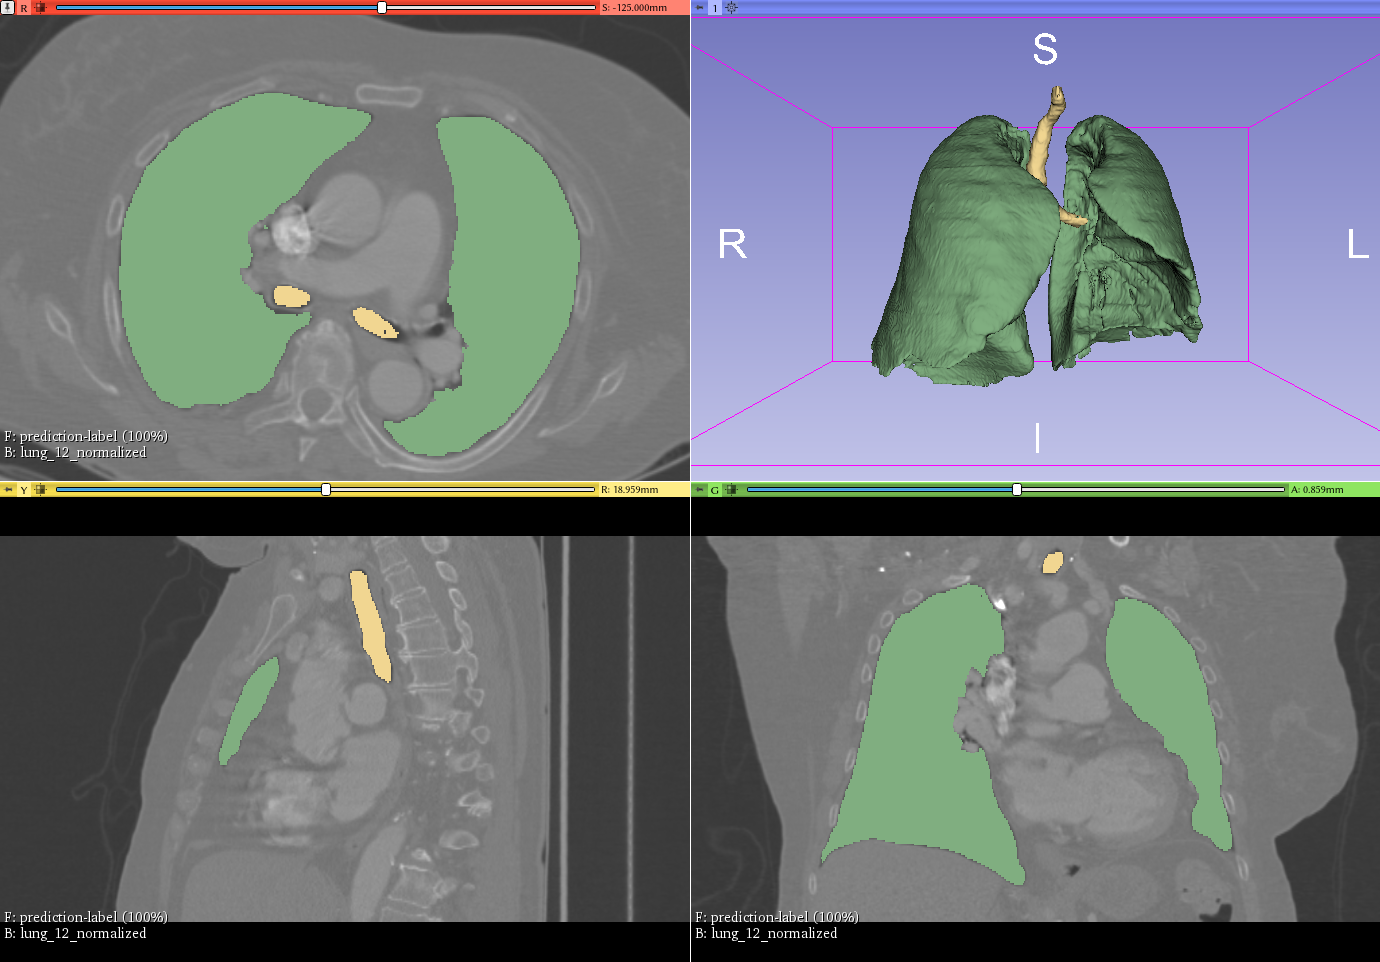
\includegraphics[width=0.49\textwidth, angle=0]{files/Fulllayoutprediction.png}
	\caption{CT scan of the lung and labeled lung (green) and the tube (yellow). The first picture represents one slice of the image, the second a 3D representation of the label and the lower two pictures are visualizations of the side and front view.}
	\label{scan_picture}
\end{figure}

The dataset consists of about 10 GB of mdh and raw files. The files contain a varying number of slices of 512 x 512 pixel grey-scale images and corresponding 512 x 512 pixel label maps. Since computational resources were limited just a subset of the data was used for this work. Furthermore the more detailed label map was reduced to one label for the lungs and one label for the tube.

\subsection{Preprocessing of image data}
Each file was converted to a NIfTI image file for better processing and visualization. These files contain all grey-scale image slices of one scan. For more appropriate input values each image was normalized ($\mu = 0.0$ and $\sigma = 1.0$) separately.
- by hand extraction

\subsection{Training and validation}

UNET
35 epochs
batch size 3 slices
adam optimizer
bce + dice loss as loss function

DEEPMEDIC
35 epochs
batch size 10 samples
learning rate 0.001 at beginning
rms propagation as optimizer and nesterov momentum with value of 0.06
l2 regularization (0.0001)
dice since it is in open source config like this



building of networks
describe it (dice loss and bce dice loss)
hold out evaluation
threshold, export files to nii.gz

\subsection{Handling huge dataset}
- ram issue
- generator solution
- still problems with data import size



